\documentclass{standalone}

\begin{document}
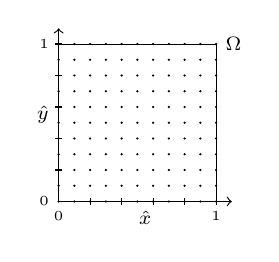
\begin{tikzpicture}
\usetikzlibrary{decorations.pathreplacing,angles,quotes}
\usetikzlibrary{shapes.geometric,shapes.misc}

    \draw[->,line width = 0.15mm]
        (0, 0) -- node[below] {\scriptsize $\hat x$} (2.2, 0);
    \draw[->,line width = 0.15mm]
        (0, 0) -- node[left] {\scriptsize $\hat y$} (0, 2.2);

    \draw[line width = 0.1mm]
        (0, 2) -- (2, 2) node[right] {\scriptsize $\Omega$} -- (2, 0);

    \foreach \x in {1,...,5}
        \draw[line width = 0.15mm]
            (0.4*\x, -0.04) -- (0.4*\x, 0.04);

    \foreach \x in {1,...,5}
        \draw[line width = 0.15mm]
            (-0.04, 0.4*\x) -- (0.04, 0.4*\x);

    \draw (0, 2) node[left] {\tiny $1$};
    \draw (0, 0) node[left] {\tiny $0$};

    \draw (2, 0) node[below] {\tiny $1$};
    \draw (0, 0) node[below] {\tiny $0$};

    \foreach \x in {0,...,10}
    \foreach \y in {0,...,10}
        \draw[fill] (0.2*\x, 0.2*\y) circle (0.005);

\end{tikzpicture}
\end{document}
